\documentclass[macfonts,phd]{njuthesis}
%% njuthesis 文档类的可选参数有:
%%   nobackinfo 取消封二页导师签名信息。注意,按照南大的规定,是需要签名页的。
%%   phd/master/bachelor 选择博士/硕士/学士论文

%%%%%%%%%%%%%%%%%%%%%%%%%%%%%%%%%%%%%%%%%%%%%%%%%%%%%%%%%%%%%%%%%%%%%%%%%%%%%%%
% 设置《国家图书馆封面》的内容,仅博士论文才需要填写

% 设置论文按照《中国图书资料分类法》的分类编号
\classification{0175.2}
% 论文的密级。需按照GB/T 7156-2003标准进行设置。预定义的值包括:
% - \openlevel,表示公开级:此级别的文献可在国内外发行和交换。
% - \controllevel,表示限制级:此级别的文献内容不涉及国家秘密,但在一定时间内
%   限制其交流和使用范围。
% - \confidentiallevel,表示秘密级:此级别的文献内容涉及一般国家秘密。
% - \clasifiedlevel,表示机密级:此级别的文献内容涉及重要的国家秘密 。
% - \mostconfidentiallevel,表示绝密级:此级别的文献内容涉及最重要的国家秘密。
% 此属性可选,默认为\openlevel,即公开级。
\securitylevel{\controllevel}
% 设置论文按照《国际十进分类法UDC》的分类编号
% 该编号可在下述网址查询:http://www.udcc.org/udcsummary/php/index.php?lang=chi
\udc{004.72}
% 国家图书馆封面上的论文标题第一行,不可换行。此属性可选,默认值为通过\title设置的标题。
\nlctitlea{博士生毕业论文}
% 国家图书馆封面上的论文标题第二行,不可换行。此属性可选,默认值为空白。
\nlctitleb{}
% 国家图书馆封面上的论文标题第三行,不可换行。此属性可选,默认值为空白。
\nlctitlec{}
% 导师的单位名称及地址
\supervisorinfo{南京大学计算机科学与技术系~~南京市汉口路22号~~210093}
% 答辩委员会主席
\chairman{XXX~~教授}
% 第一位评阅人
\reviewera{XXX~~教授}
% 第二位评阅人
\reviewerb{XXX~~副教授}
% 第三位评阅人
\reviewerc{XXX~~教授}
% 第四位评阅人
\reviewerd{XXX~~研究员}

\newcommand{\kaiti}[1]{{\kaishu{#1}}}

\def\A{{\boldsymbol A}}
\def\a{{\boldsymbol a}}
\def\B{{\boldsymbol B}}
\def\b{{\boldsymbol b}}
\def\C{{\boldsymbol C}}
\def\c{{\boldsymbol c}}
\def\D{{\boldsymbol D}}
\def\d{{\boldsymbol d}}
\def\E{{\boldsymbol E}}
\def\e{{\boldsymbol e}}
\def\F{{\boldsymbol F}}
\def\f{{\boldsymbol f}}
\def\G{{\boldsymbol G}}
\def\g{{\boldsymbol g}}
\def\H{{\boldsymbol H}}
\def\h{{\boldsymbol h}}
\def\I{{\boldsymbol I}}
\def\i{{\boldsymbol i}}
\def\J{{\boldsymbol J}}
\def\j{{\boldsymbol j}}
\def\K{{\boldsymbol K}}
\def\k{{\boldsymbol k}}
\def\L{{\boldsymbol L}}
\def\l{{\boldsymbol l}}
\def\M{{\boldsymbol M}}
\def\m{{\boldsymbol m}}
\def\N{{\boldsymbol N}}
\def\n{{\boldsymbol n}}
\def\O{{\boldsymbol O}}
\def\o{{\boldsymbol o}}
\def\P{{\boldsymbol P}}
\def\p{{\boldsymbol p}}
\def\Q{{\boldsymbol Q}}
\def\q{{\boldsymbol q}}
\def\R{{\boldsymbol R}}
\def\r{{\boldsymbol r}}
\def\S{{\boldsymbol S}}
\def\s{{\boldsymbol s}}
\def\T{{\boldsymbol T}}
\def\t{{\boldsymbol t}}
\def\U{{\boldsymbol U}}
\def\u{{\boldsymbol u}}
\def\V{{\boldsymbol V}}
\def\v{{\boldsymbol v}}
\def\W{{\boldsymbol W}}
\def\w{{\boldsymbol w}}
\def\X{{\boldsymbol X}}
\def\x{{\boldsymbol x}}
\def\Y{{\boldsymbol Y}}
\def\y{{\boldsymbol y}}
\def\Z{{\boldsymbol Z}}
\def\z{{\boldsymbol z}}

\def\AM{{\mathcal A}}
\def\BM{{\mathcal B}}
\def\CM{{\mathcal C}}
\def\DM{{\mathcal D}}
\def\EM{{\mathcal E}}
\def\FM{{\mathcal F}}
\def\GM{{\mathcal G}}
\def\HM{{\mathcal H}}
\def\IM{{\mathcal I}}
\def\JM{{\mathcal J}}
\def\KM{{\mathcal K}}
\def\LM{{\mathcal L}}
\def\MM{{\mathcal M}}
\def\NM{{\mathcal N}}
\def\OM{{\mathcal O}}
\def\PM{{\mathcal P}}
\def\QM{{\mathcal Q}}
\def\RM{{\mathcal R}}
\def\SM{{\mathcal S}}
\def\TM{{\mathcal T}}
\def\UM{{\mathcal U}}
\def\VM{{\mathcal V}}
\def\WM{{\mathcal W}}
\def\XM{{\mathcal X}}
\def\YM{{\mathcal Y}}
\def\ZM{{\mathcal Z}}

\def\AB{{\mathbb A}}
\def\BB{{\mathbb B}}
\def\CB{{\mathbb C}}
\def\DB{{\mathbb D}}
\def\EB{{\mathbb E}}
\def\FB{{\mathbb F}}
\def\GB{{\mathbb G}}
\def\HB{{\mathbb H}}
\def\IB{{\mathbb I}}
\def\JB{{\mathbb J}}
\def\KB{{\mathbb K}}
\def\LB{{\mathbb L}}
\def\MB{{\mathbb M}}
\def\NB{{\mathbb N}}
\def\OB{{\mathbb O}}
\def\PB{{\mathbb P}}
\def\QB{{\mathbb Q}}
\def\RB{{\mathbb R}}
\def\SB{{\mathbb S}}
\def\TB{{\mathbb T}}
\def\UB{{\mathbb U}}
\def\VB{{\mathbb V}}
\def\WB{{\mathbb W}}
\def\XB{{\mathbb X}}
\def\YB{{\mathbb Y}}
\def\ZB{{\mathbb Z}}

\def\tanh{\text{tanh}}
\def\sgn{\text{sign}}
\def\diag{\text{diag}}
\def\svd{\text{svd}}
\def\st{\text{subject to:}}
\def\sigmoid{\text{sigmoid}}
\def\con{\text{con}}

\def\bone{{\bf 1}}
\def\bzero{{\bf 0}}

\def\hone{{\mathds{1}}}
\def\hzero{{\mathds{0}}}

\def\ph{\mbox{\boldmath$\phi$\unboldmath}}
\def\Pii{\mbox{\boldmath$\Pi$\unboldmath}}
\def\pii{\mbox{\boldmath$\pi$\unboldmath}}
\def\Ph{\mbox{\boldmath$\Phi$\unboldmath}}
\def\Ps{\mbox{\boldmath$\Psi$\unboldmath}}
\def\tha{\mbox{\boldmath$\theta$\unboldmath}}
\def\muu{\mbox{\boldmath$\mu$\unboldmath}}
\def\Si{\mbox{\boldmath$\Sigma$\unboldmath}}
\def\Gam{\mbox{\boldmath$\Gamma$\unboldmath}}
\def\Lam{\mbox{\boldmath$\Lambda$\unboldmath}}
\def\De{\mbox{\boldmath$\Delta$\unboldmath}}
\def\vps{\mbox{\boldmath$\varepsilon$\unboldmath}}
\def\Lap{\mbox{\boldmath$\LM$\unboldmath}}
\newcommand{\ti}[1]{\tilde{#1}}

\newcommand{\sota}[1]{{\bf #1}}
\newcommand{\sebe}[1]{{\underline{#1}}}


\def\tr{\text{tr}}
\def\dist{\text{dist}}
\def\const{\text{const}}
\def\bias{\text{bias}}
\def\etal{{\em et al.\/}\,}
\newcommand{\indep}{{\;\bot\!\!\!\!\!\!\bot\;}}
\def\argmax{\mathop{\rm argmax}}
\def\argmin{\mathop{\rm argmin}}

\def\dg{\text{diag}}
\newcommand{\bigO}[1]{\ensuremath{\operatorname{\OM}\left(#1\right)}}



\usepackage{amsthm}
\usepackage{amsmath}
\usepackage{amssymb}
\usepackage{array}
\usepackage{algorithm}
\usepackage{algorithmic}

\usepackage{color}

\usepackage{dashrule}
\usepackage{dsfont}

\usepackage{eufrak}

\usepackage{fontspec}

\usepackage{graphicx}

\usepackage{longtable}

\usepackage{makecell}

\usepackage{pgfplots}

\usepackage{relsize}

\usepackage{tikz}

\usetikzlibrary{calc}
\usetikzlibrary{backgrounds}
\usetikzlibrary{positioning,shadows}
\usetikzlibrary{arrows.meta}

\usepackage[utf8]{inputenc}

\def\TBD{{\color{red}{TBD}}}

\floatname{algorithm}{算法} 
\renewcommand{\algorithmicrequire}{\textbf{输入:}}
\renewcommand{\algorithmicensure}{\textbf{输出:}}

\newcolumntype{Z}[1]{>{\centering\let\newline\\\arraybackslash\hspace{0pt}}m{#1}}
\newcolumntype{L}[1]{>{\let\newline\\\arraybackslash\hspace{0pt}}m{#1}}

\newcommand{\tabincell}[2]{\begin{tabular}{@{}#1@{}}#2\end{tabular}} 


%%%%%%%%%%%%%%%%%%%%%%%%%%%%%%%%%%%%%%%%%%%%%%%%%%%%%%%%%%%%%%%%%%%%%%%%%%%%%%%
% 设置论文的中文封面

% 论文标题,不可换行
% \title{博士生毕业论文}
% 如果论文标题过长,可以分两行,第一行用\titlea{}定义,第二行用\titleb{}定义,将上面的\title{}注释掉
\titlea{博士生毕业论文}
\titleb{}

% 论文作者姓名
\author{XXX}
% 论文作者联系电话
\telphone{159-xxxx-xxxx}
% 论文作者电子邮件地址
\email{xxx@nju.edu.cn}
% 论文作者学生证号
\studentnum{DGxxxxxxx}
% 论文作者入学年份(年级)
\grade{2016}
% 导师姓名职称
\supervisor{XXX~~教授}
% 导师的联系电话
\supervisortelphone{159-xxxx-xxxx}
% 论文作者的学科与专业方向
\major{计算机科学与技术}
% 论文作者的研究方向
\researchfield{研究领域}
% 论文作者所在院系的中文名称
\department{计算机科学与技术系}
% 论文作者所在学校或机构的名称。此属性可选,默认值为``南京大学''。
\institute{南京大学}
% 论文的提交日期,需设置年、月、日。
\submitdate{20xx年x月xx日}
% 论文的答辩日期,需设置年、月、日。
\defenddate{20xx年x月xx日}
% 论文的定稿日期,需设置年、月、日。此属性可选,默认值为最后一次编译时的日期,精确到日。
%% \date{2013年5月1日}

%%%%%%%%%%%%%%%%%%%%%%%%%%%%%%%%%%%%%%%%%%%%%%%%%%%%%%%%%%%%%%%%%%%%%%%%%%%%%%%
% 设置论文的英文封面

% 论文的英文标题,不可换行
\englishtitle{Research Field}
% 论文作者姓名的拼音
\englishauthor{XXX}
% 导师姓名职称的英文
\englishsupervisor{Professor XXX}
% 论文作者学科与专业的英文名
\englishmajor{Computer Science and Technology}
% 论文作者所在院系的英文名称
\englishdepartment{Department of Computer Science and Technology}
% 论文作者所在学校或机构的英文名称。此属性可选,默认值为``Nanjing University''。
\englishinstitute{Nanjing University}
% 论文完成日期的英文形式,它将出现在英文封面下方。需设置年、月、日。日期格式使用美国的日期
% 格式,即``Month day, year'',其中``Month''为月份的英文名全称,首字母大写;``day''为
% 该月中日期的阿拉伯数字表示;``year''为年份的四位阿拉伯数字表示。此属性可选,默认值为最后
% 一次编译时的日期。
\englishdate{September 1, 2020}

%%%%%%%%%%%%%%%%%%%%%%%%%%%%%%%%%%%%%%%%%%%%%%%%%%%%%%%%%%%%%%%%%%%%%%%%%%%%%%%
% 设置论文的中文摘要

% 设置中文摘要页面的论文标题及副标题的第一行。
% 此属性可选,其默认值为使用|\title|命令所设置的论文标题
\abstracttitlea{博士生毕业论文}
% 设置中文摘要页面的论文标题及副标题的第二行。
% 此属性可选,其默认值为空白
\abstracttitleb{}

%%%%%%%%%%%%%%%%%%%%%%%%%%%%%%%%%%%%%%%%%%%%%%%%%%%%%%%%%%%%%%%%%%%%%%%%%%%%%%%
% 设置论文的英文摘要

% 设置英文摘要页面的论文标题及副标题的第一行。
% 此属性可选,其默认值为使用|\englishtitle|命令所设置的论文标题
\englishabstracttitlea{PhD. Thesis}
% 设置英文摘要页面的论文标题及副标题的第二行。
% 此属性可选,其默认值为空白
\englishabstracttitleb{}

%%%%%%%%%%%%%%%%%%%%%%%%%%%%%%%%%%%%%%%%%%%%%%%%%%%%%%%%%%%%%%%%%%%%%%%%%%%%%%%
\begin{document}

%%%%%%%%%%%%%%%%%%%%%%%%%%%%%%%%%%%%%%%%%%%%%%%%%%%%%%%%%%%%%%%%%%%%%%%%%%%%%%%

% 制作国家图书馆封面(博士学位论文才需要)
\makenlctitle
% 制作中文封面
\maketitle
% 制作英文封面
\makeenglishtitle


%%%%%%%%%%%%%%%%%%%%%%%%%%%%%%%%%%%%%%%%%%%%%%%%%%%%%%%%%%%%%%%%%%%%%%%%%%%%%%%
% 开始前言部分
\frontmatter

%%%%%%%%%%%%%%%%%%%%%%%%%%%%%%%%%%%%%%%%%%%%%%%%%%%%%%%%%%%%%%%%%%%%%%%%%%%%%%%
% 论文的中文摘要
\begin{abstract}
这里是摘要。
\keywords{关键词1}
\end{abstract}

%%%%%%%%%%%%%%%%%%%%%%%%%%%%%%%%%%%%%%%%%%%%%%%%%%%%%%%%%%%%%%%%%%%%%%%%%%%%%%%
% 论文的英文摘要
\begin{englishabstract}
This is abstract.
\englishkeywords{Keywords}
\end{englishabstract}

% %%%%%%%%%%%%%%%%%%%%%%%%%%%%%%%%%%%%%%%%%%%%%%%%%%%%%%%%%%%%%%%%%%%%%%%%%%%%%%%
% % 论文的前言,应放在目录之前,中英文摘要之后
% %
\begin{preface}
\noindent{\bf 前言}

\noindent{\bf 公式符号校对:}
\begin{itemize}
\item $abcdefghijklmnopqrstuvwxyz$
\item $\bf{abcdefghijklmnopqrstuvwxyz}$
\item $\boldsymbol{abcdefghijklmnopqrstuvwxyz}$
\item $ABCDEFGHIJKLMNOPQRSTUVWXYZ$
\item $\bf{ABCDEFGHIJKLMNOPQRSTUVWXYZ}$
\item $\boldsymbol{ABCDEFGHIJKLMNOPQRSTUVWXYZ}$
\item $\mathcal{ABCDEFGHIJKLMNOPQRSTUVWXYZ}$
\item $\mathbb{ABCDEFGHIJKLMNOPQRSTUVWXYZ}$
\item $\alpha\beta\gamma\delta\epsilon\eta\theta\iota\kappa\lambda\mu\nu\xi\pi\rho\sigma\tau\upsilon\phi\chi\psi\omega$
\item $\Gamma\Delta\Theta\Lambda\Xi\Phi\Pi\Sigma\Upsilon\Psi\Omega$
\end{itemize}

\begin{flushright}
XXX\\
20XX年夏于南京大学
\end{flushright}
\end{preface}

%%%%%%%%%%%%%%%%%%%%%%%%%%%%%%%%%%%%%%%%%%%%%%%%%%%%%%%%%%%%%%%%%%%%%%%%%%%%%%%
% 生成论文目次
\tableofcontents

%%%%%%%%%%%%%%%%%%%%%%%%%%%%%%%%%%%%%%%%%%%%%%%%%%%%%%%%%%%%%%%%%%%%%%%%%%%%%%%
% 生成插图清单。如无需插图清单则可注释掉下述语句。
\listoffigures

%%%%%%%%%%%%%%%%%%%%%%%%%%%%%%%%%%%%%%%%%%%%%%%%%%%%%%%%%%%%%%%%%%%%%%%%%%%%%%%
% 生成附表清单。如无需附表清单则可注释掉下述语句。
\listoftables

%%%%%%%%%%%%%%%%%%%%%%%%%%%%%%%%%%%%%%%%%%%%%%%%%%%%%%%%%%%%%%%%%%%%%%%%%%%%%%%
% 开始正文部分
\mainmatter

%%%%%%%%%%%%%%%%%%%%%%%%%%%%%%%%%%%%%%%%%%%%%%%%%%%%%%%%%%%%%%%%%%%%%%%%%%%%%%%

%% chapter0:模板
\chapter{模板}
\section{常用结构模板}

\subsection{引用示例}
书籍:模式识别\cite{PRML:books/BishopCM/2006}。

会议论文:隐狄利克雷分布特征\cite{LDA:conf/nips/BleiNJ01}(Latent Dirichlet Allocation, 简称 LDA)。

博士毕业论文:离散二次规划\cite{BQP:phdthesis/Yang13}。

期刊论文:乘积量化\cite{PQ:journals/pami/JegouDS11}(Product Quantization, 简称PQ)。

\subsection{表格示例}
表\ref{tab:template-example}~给出了表格的示例。

%---------------table starts---------------
\begin{table*}[h]
\centering
\caption{XXX方法的性能}
\label{tab:template-example}
\begin{tabular}{rc}
\toprule
方法   &   精度    \\\midrule
XX    & \sebe{0.1111}   \\
XY    & \sota{0.9999}   \\
\bottomrule
\end{tabular}
\end{table*}
%---------------table ends---------------

\subsection{插图示例}
图\ref{fig:template-example}~给出了插图的示例。


\begin{figure}[h]\centering
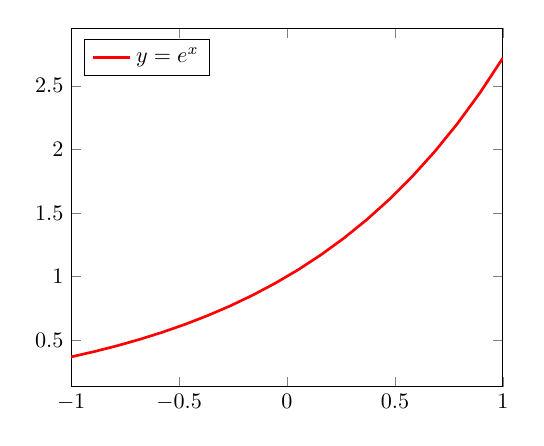
\begin{tikzpicture}[scale=0.8]
	\begin{axis}[legend pos=north west,xmin=-1, xmax=1,legend cell align={left},]
	\addplot[color=red, line width=1.2pt,samples=20,domain=-1:1] {e^x};\addlegendentry{$y=e^x$}
	\end{axis}
\end{tikzpicture}
\caption{XXX方法的性能}
\label{fig:template-example}
\end{figure}


%% chapter1:绪论
\chapter{绪论}\label{chp:intro}
\section{引言}\label{sec:intro}
这里是绪论引言。
\section{有待研究的问题}\label{sec:problems}
这里是有待研究的问题。
\section{本文工作}\label{sec:works}
这里是本文工作。
\section{论文组织}\label{sec:problems}
论文组织示意图如图\ref{fig:chp1-logic}~所示。
\begin{figure}[h]\centering
\tikz \node [scale=0.65, inner sep=0] {
\tikzset{%
  >={Latex[width=2mm,length=2mm]},
  % Specifications for style of nodes:
            base/.style = {rectangle, rounded corners, draw={rgb:red,4;yellow,2},
                            text width=4cm, minimum height=1.75cm,
                            text centered,
                            copy shadow={draw, fill={rgb:red,4;yellow,2}, 
                            shadow xshift=-1.5mm, shadow yshift=1.5mm}},
        category/.style = {rectangle, rounded corners, draw={rgb:orange,2;yellow,2},
                            text width=3.75cm, minimum height=2cm,
                            text centered,
                            copy shadow={draw, fill={rgb:orange,2;yellow,2}, 
                            shadow xshift=-1.5mm, shadow yshift=1.5mm}},
           model/.style = {rectangle, rounded corners, draw=black!30!green,
                            text width=3.75cm, minimum height=2cm,
                            text centered,
                            copy shadow={draw, fill=black!30!green, 
                            shadow xshift=-1.5mm, shadow yshift=1.5mm}},
          method/.style = {rectangle, rounded corners, draw={rgb:red,4;green,1},
                            text width=3.75cm, minimum height=1.75cm,
                            text centered,
                            copy shadow={draw, fill={rgb:red,4;green,1}, 
                            shadow xshift=-1.5mm, shadow yshift=1.5mm}},
}
\begin{tikzpicture}[framed, background rectangle/.style={draw=gray!15, bottom color=gray!15, top color=gray!15, rounded corners}, 
    node distance=3.5cm,
    every node/.style={fill=white, font=\sffamily\large}, align=center]
  % Specification of nodes (position, etc.)
  \node (thesis)            [base, line width=0.5mm]                                                      
                            {毕业论文};
  %%%%%%%%%%%%%%%%%%%%%%%%%%%%%%%%%%%%%%%%%%%%%%%%%%                          
  \node (cate1)             [category, below of=thesis, xshift=-5cm, line width=0.5mm]
                            {归档1};
  \node (cate2)             [category, below of=thesis, xshift=5cm, line width=0.5mm]
                            {归档2};
  %%%%%%%%%%%%%%%%%%%%%%%%%%%%%%%%%%%%%%%%%%%%%%%%%%                          
  \node (model1)            [model, below of=cate1, xshift=-2.25cm, line width=0.5mm]
                            {模型1};         
  \node (model2)            [model, below of=cate1, xshift=2.25cm, line width=0.5mm]
                            {模型2};    
  \node (model3)            [model, below of=cate2, xshift=-2.25cm, line width=0.5mm]
                            {模型3};
  \node (model4)            [model, below of=cate2, xshift=2.25cm, line width=0.5mm]
                            {模型4};
  %%%%%%%%%%%%%%%%%%%%%%%%%%%%%%%%%%%%%%%%%%%%%%%%%%                          
  \node (method1)           [method, below of=model1, line width=0.5mm]  
                            {方法1};
  \node (method2)           [method, below of=model2, line width=0.5mm]  
                            {方法2};
  \node (method3)           [method, below of=model3, line width=0.5mm]  
                            {方法3};
  \node (method4)           [method, below of=model4, line width=0.5mm]  
                            {方法4};
]
\draw[line width=0.5mm, color=gray!15]                                             (-9.35,-11.5) -- (-9.35,1.25);
\draw[line width=0.5mm, color=gray!15]                                                   (-9.5,1.2) -- (9.5,1.2);
\draw[line width=0.5mm, color={rgb:red,4;yellow,2}]                                         (thesis) -- (0,-1.5);
\draw[-{>[scale=1.5]}, line width=0.5mm, color={rgb:red,4;yellow,2}]                      (0,-1.5) -| (-5,-2.25);
\draw[-{>[scale=1.5]}, line width=0.5mm, color={rgb:red,4;yellow,2}]                       (0,-1.5) -| (5,-2.25);
\draw[line width=0.5mm, color={rgb:orange,2;yellow,2}]                                     (cate1) -- (-5,-5.25);
\draw[line width=0.5mm, color={rgb:orange,2;yellow,2}]                                      (cate2) -- (5,-5.25);
\draw[-{>[scale=1.5]}, line width=0.5mm, color={rgb:orange,2;yellow,2}]              (-5,-5.25) -| (-2.75,-5.85);
\draw[-{>[scale=1.5]}, line width=0.5mm, color={rgb:orange,2;yellow,2}]              (-5,-5.25) -| (-7.25,-5.85);
\draw[-{>[scale=1.5]}, line width=0.5mm, color={rgb:orange,2;yellow,2}]                (5,-5.25) -| (2.75,-5.85);
\draw[-{>[scale=1.5]}, line width=0.5mm, color={rgb:orange,2;yellow,2}]                (5,-5.25) -| (7.25,-5.85);
\draw[-{>[scale=1.5]}, line width=0.5mm, color=black!30!green]                         (model1) -- (-7.25,-9.35);
\draw[-{>[scale=1.5]}, line width=0.5mm, color=black!30!green]                         (model2) -- (-2.75,-9.35);
\draw[-{>[scale=1.5]}, line width=0.5mm, color=black!30!green]                          (model3) -- (2.75,-9.35);
\draw[-{>[scale=1.5]}, line width=0.5mm, color=black!30!green]                          (model4) -- (7.25,-9.35);
\end{tikzpicture}
};
\caption{论文组织}
\label{fig:chp1-logic}
\end{figure}




%% chapter2:相关工作
\chapter{相关工作}\label{chp:related-work}
\section{XXX领域发展现状}\label{sec:development}
这里是领域发展现状。

%% chapter3:方法1
\chapter{方法1}\label{chp:method1}
\section{引言}
这里是方法1引言。
\section{问题定义}
这里是问题定义。
\section{方法1}
\subsection{模型}
这里是方法1模型。
\subsection{学习算法}
这里是方法1学习算法。
\section{实验测试}
这里是实验测试。
\subsection{数据集}
这里是数据集。
\subsection{实验设置}
这里是实验设置。
\subsection{性能对比}
这里是性能对比。
\subsection{超参数敏感性实验}
这里是超参数敏感性实验。
\section{总结}
这里是总结。


%% chapter4:总结与展望
\chapter{总结与展望}
\section{本文总结}
这里是本文总结。
\section{未来工作展望}
这里是未来工作展望。

% 参考文献。应放在\backmatter之前。
% 推荐使用BibTeX,若不使用BibTeX时注释掉下面一句。
% \nocite{*} % 有这个命令的话,未引用的参考文献,只要出现在bib中,都将出现在引用列表中
\bibliography{sample}
% 附录,必须放在参考文献后,backmatter前

\begin{acknowledgement}
致谢。
\end{acknowledgement}

\appendix
\chapter{符号及简称说明}\label{chp:appendix}
\section{本文使用的符号}
表\ref{tab:appendix-notaions}中列出了一些本文使用的通用符号。
\begin{table}[H]
\centering
\caption{本文使用的符号}
\label{tab:appendix-notaions}
\begin{tabular}{ll}
\toprule
符号                    &    说明                                    \\\midrule
$\varnothing$          &    空集                                    \\
$\RB$                  &    实空间                                   \\
$\RB^c$                &    $c$维实空间                              \\ 
$\{-1,+1\}^c$          &    $c$维二值空间                            \\
$\B$                   &    大写黑体字母,矩阵                        \\
$\B_{i*}$              &    矩阵$\B$的第$i$行                        \\
$\B_{*j}$              &    矩阵$\B$的第$j$列                        \\
$B_{ij}$               &    矩阵$\B$中行标为$i$,列标为$j$的元素        \\
$\b$                   &    小写黑体字母,列向量                       \\
$b_i$                  &    向量$\b_i$的第$i$个元素                   \\
$\I_n$                 &    维度为$n\times n$的单位矩阵               \\
$\bone_d$              &    元素全部为1的$d$维向量                    \\
$\bone_{n\times n}$    &    元素全部为1的$n\times n$的矩阵            \\
$\bzero_d$             &    元素全部为0的$d$维向量                    \\
$\bzero_{n\times n}$   &    元素全部为0的$n\times n$的矩阵            \\
$\B^\top$              &    矩阵$\B$的转置                           \\
$\B\succeq\bzero$      &    半正定矩阵                               \\
$\A\succeq\B$          &    矩阵$\A-\B$为半正定矩阵                   \\
$\B\succ\bzero$        &    正定矩阵                                \\
$\A\succ\B$            &    矩阵$\A-\B$为正定矩阵                    \\
\bottomrule
\end{tabular}
\end{table}

此外,一些函数定义如下。
\begin{itemize}
\item 矩阵的迹:
\begin{align}
\tr(\B)=\sum_{i=1}^nB_{ii}.\label{fun:appendix-trace}
\end{align}
\item 向量的2范数:
\begin{align}
\Vert\b\Vert_2=\sqrt{\sum_{i=1}^nb_i^2}.\label{fun:appendix-2norm}
\end{align}
\item 矩阵的Frobenius范数:
\begin{align}
\Vert\B\Vert_F=\sqrt{\sum_{i,j=1}^nB_{ij}^2}.\label{fun:appendix-Fnorm}
\end{align}
\item 矩阵的1范数:
\begin{align}
\Vert\B\Vert_1=\sum_{i,j=1}^n\vert B_{ij}\vert.\label{fun:appendix-1norm}
\end{align}
\item 指示函数:
\begin{align}
\hone(condition)=\left\{
\begin{array}{ll}
1   & \text{if } condition \text{ is true},\\
0   & \text{otherwise.}
\end{array}
\right.\label{fun:appendix-indicator}
\end{align}
\end{itemize}

\section{简称说明}
表\ref{tab:appendix-abbr}列出了一些本文使用的简称的含义。
\begin{longtable}{ll}
\caption{本文使用的通用简称}
\label{tab:appendix-abbr}
\endfirsthead
\endhead
\toprule
简称         & 全称                                                   \\\midrule
BQP         & Binary Quadratic Programming,离散二次规划               \\
PQ          & Product Quantization,乘积量化                          \\
\bottomrule
\end{longtable}



%%%%%%%%%%%%%%%%%%%%%%%%%%%%%%%%%%%%%%%%%%%%%%%%%%%%%%%%%%%%%%%%%%%%%%%%%%%%%%%
% 书籍附件
\backmatter
%%%%%%%%%%%%%%%%%%%%%%%%%%%%%%%%%%%%%%%%%%%%%%%%%%%%%%%%%%%%%%%%%%%%%%%%%%%%%%%
% 作者简历与科研成果页,应放在backmatter之后
\begin{resume}
% 论文作者身份简介,一句话即可。
\begin{authorinfo}
\noindent XXX,男,汉族,XXXX年XX月出生,云南省腾冲市人。
\end{authorinfo}
% 论文作者教育经历列表,按日期从近到远排列,不包括将要申请的学位。
\begin{education}
\item[20XX年X月 --- 20XX年X月] 南京大学计算机科学与技术系 \hfill 本科
\end{education}
\begin{award}
\item 荣誉1
\end{award}

% 论文作者在攻读学位期间所发表的文章的列表,按发表日期从近到远排列。
\begin{publications}
\item \underline{XXX}, XXX. Title 1[C] //Proceedings of the XXX. 20XX: xxxx–xxxx. {\bf (CCF-A 类会议)}
\end{publications}
\begin{patent}
\item {xxx\kaiti{xxx}。}{一种XXX方法}。{专利号:XXX.X}
\end{patent}
% 论文作者在攻读学位期间参与的科研课题的列表,按照日期从近到远排列。
% \begin{projects}
% \item 国家自然科学基金面上项目``无线传感器网络在知识获取过程中的若干安全问题研究''
% (课题年限~2010年1月 --- 2012年12月),负责位置相关安全问题的研究。
% \end{projects}
\end{resume}

%%%%%%%%%%%%%%%%%%%%%%%%%%%%%%%%%%%%%%%%%%%%%%%%%%%%%%%%%%%%%%%%%%%%%%%%%%%%%%%
% 生成《学位论文出版授权书》页面,应放在最后一页
\makelicense

%%%%%%%%%%%%%%%%%%%%%%%%%%%%%%%%%%%%%%%%%%%%%%%%%%%%%%%%%%%%%%%%%%%%%%%%%%%%%%%
\end{document}

